\section{Validation}
\label{sec:validation}

\subsection{CronometroPSP: A Real System, Fully Specified}
\label{sec:cronometro-spec}

The primary validation of Trenza is the complete formal specification of
CronometroPSP---the application that motivated the language's design. The
specification comprises sixteen \texttt{.trz} source files, of which thirteen
are behavioral contexts organized in three layers:

\begin{sloppypar}
\begin{itemize}
  \item \textbf{Base layer}: \texttt{NormalMode} (initial context) and
        \texttt{EditMode}.
  \item \textbf{Concurrent layer}: \texttt{ActiveSession}---active while a task
        session is running.
  \item \textbf{Overlay layer}: ten modal contexts---\texttt{ConfigMenu},
        \texttt{Comment\-Modal}, \texttt{Create\-Task\-Modal},
        \texttt{Edit\-Task\-Modal}, \texttt{Edit\-Activity\-Modal},
        \texttt{Create\-Activity\-Modal}, \texttt{Select\-Activity\-Modal},
        \texttt{History\-Modal}, \texttt{ResetModal}, \texttt{About\-Modal}.
\end{itemize}
\end{sloppypar}

The complete specification is verified by all eight rules in under one hundred
milliseconds. Multi-strand synthesis from the same source produces 1,107 lines
of Rust, 942 lines of Rust tests, 1,061 lines of TypeScript, and 978 lines of
TypeScript tests---four target files from sixteen sources, all derived and
therefore guaranteed consistent.

\begin{table*}[t]
  \centering
  \caption{CronometroPSP reference specification: compilation metrics.
           All values verified from generated outputs in
           \texttt{spec/reference/cronometro-psp/generated/}~\cite{trenza2026repo}.}
  \label{tab:metrics}
  \small
  \begin{tabular}{lrlr}
    \toprule
    \textbf{Metric} & \textbf{Value} & \textbf{Metric} & \textbf{Value} \\
    \midrule
    \texttt{.trz} source files & 16    & Verification time     & $<100$\,ms \\
    Behavioral contexts        & 13    & Rust LOC (generated)  & 1{,}107    \\
    Distinct event handlers    & 35    & Rust test LOC         &   942      \\
    Transitions (schematic)    & 45    & TypeScript LOC        & 1{,}061    \\
    Mermaid schematic lines    & 47    & TypeScript test LOC   &   978      \\
    \bottomrule
  \end{tabular}
\end{table*}

\begin{figure*}[t]
  \centering
  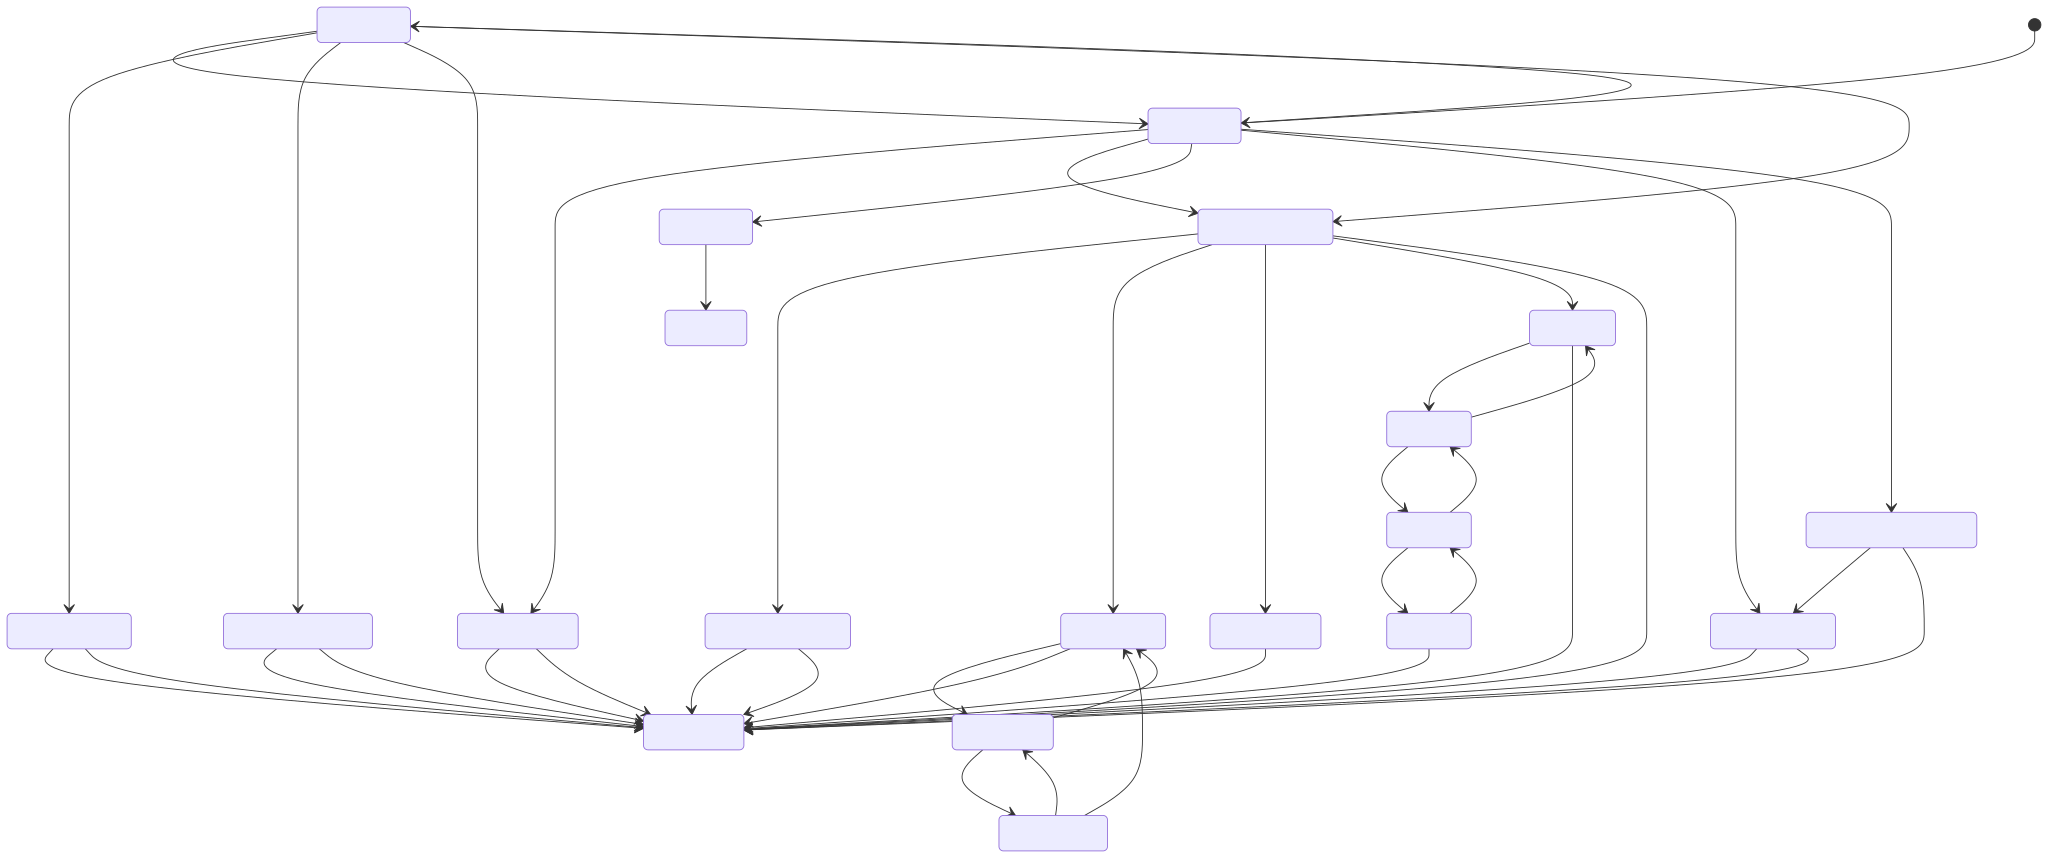
\includegraphics[width=\textwidth]{figures/cronometro_psp}
  \caption{Generated statechart for CronometroPSP: thirteen behavioral contexts
           organized in base, concurrent, and overlay layers. Produced by
           Strand~3 of the Trenza compiler from the sixteen \texttt{.trz}
           source files.}
  \label{fig:cronometro}
\end{figure*}

The specification exercise was not merely a validation of the toolchain. It
was a diagnostic of the original system. During the process of writing all
thirteen behavioral context files, eight gaps in the language's expressiveness
were identified---design properties that the original application required but
that the DSL could not yet represent. The most significant was the absence of
typed context parameters: when \texttt{EditMode} transitions to
\texttt{EditTaskModal}, it needs to pass the identifier of the task being
edited. Without this mechanism, the information travels as implicit global
state---exactly the \texttt{AppState.pendingTaskId} pattern that Trenza was
designed to eliminate.

The gaps were not failures of the specification process. They were its product.
Attempting to formally specify a real system revealed, with precision, the
boundaries of what the language could express. Each gap became a design
requirement for the next iteration. The CronometroPSP exercise is, in this
sense, evidence that the language is alive: it found its own limits by being
used.

\subsection{Self-Hosting}
\label{sec:selfhosting}

The CLI tool that verifies and generates Trenza specifications is itself
specified in Trenza. The \texttt{trenza-cli.trz} file describes the CLI's own
behavioral contexts: the valid sequences of commands, the states the tool can
be in (parsing, verifying, generating, reporting), and the transitions between
them. Self-hosting was verified on 24 March 2026.

Self-hosting has a specific meaning in this context: it is not that the tool is
written in its own language, but that the tool's behavior is governed by a
specification that the tool itself can verify. If the CLI violates its own
specification, the verifier will report the violation. The tool cannot be
inconsistent with itself without the inconsistency being detectable.

This is a completeness argument, not a performance benchmark. It demonstrates
that the language is expressive enough to describe at least one real, non-trivial
software tool---and that the verification infrastructure is robust enough to
apply to its own governance.

\subsection{Multi-LLM Collaboration as Evidence}
\label{sec:collab-evidence}

The development history of Trenza is itself a validation of the collaboration
model described in Section~\ref{sec:collaboration}. Three models participated
in the design: Claude Sonnet~4.6 for session coordination and specification,
Claude Opus~4.6 for architectural review, and Gemini~3.1 Pro for adversarial
challenge and independent implementation of the Rust compiler (with the bulk
of implementation throughput delivered by Gemini~3 Flash under Pro's quota
constraints).

The most concrete evidence is \textbf{Rule~8 (role-type consistency)}, added
by a Gemini~3 Flash session during self-hosting work---without prompting from the
human or from the larger model---because the formal specification made the gap
visible by inspection. The full account is in Section~\ref{sec:roles}; the
point here is structural: the collaboration produced the verification rule that
was necessary, from the model that was positioned to see the need, because the
specification was precise enough to make the gap nameable.

\subsection{What Remains}
\label{sec:remains}

The toolchain described in Section~\ref{sec:language} is functional but not
complete. The gap analysis from Section~\ref{sec:cronometro-spec} identified
design properties that the language does not yet express---most notably typed
context parameters for passing data across transitions without global state.
MonitoreoRed remains without a \texttt{.trz} specification.

These are not qualifications of the thesis. They are the expected state of a
language at version~0.0.1. The claim is not that Trenza is finished. The claim
is that the structural approach---formal constraint as the response to state
dispersal---is validated by the cases where it has been applied, and that the
gaps it exposes are more useful than the silence of an undisciplined system.
